\pagebreak
\section{Motor Tests - Friction} \label{app:motorTestFriction}
\textbf{Name: Group 510}\\
\textbf{Date: 30/09 - 2015}

\subsubsection{Purpose}
The purpose of the test is to find the motor friction, B, by measuring the motor current and the corresponding velocities, in several steady states.

\textbf{The data from the test \textit{Generator Constant} is reused, the equipment and setup is then the same.}

\subsubsection{Results}
%
\begin{table}[H]
\begin{tabular}{|l|l|l| l|l|}
\cline{1-2}\cline{4-5}%-------------------------             -------------------------------------------------
  \textbf{Input (A)}   & \textbf{Output (RPM)} &\phantom{hey}& \textbf{Input (A)}   & \textbf{Output (RPM)} \\
\cline{1-2}\cline{4-5}%-------------------------             -------------------------------------------------
  1,7                &             $3684$    &             & 4,1                & $21966$               \\
\cline{1-2}\cline{4-5}%-------------------------             -------------------------------------------------
  2,2                &             $8063$    &             & 4,8                & $26420$               \\
\cline{1-2}\cline{4-5}%-------------------------             -------------------------------------------------
  2,6                &             $12021$   &             & 5,6                & $31447$               \\
\cline{1-2}\cline{4-5}%-------------------------             -------------------------------------------------
  3,3                &             $16746$  \\
\cline{1-2}%------------------------------------
\end{tabular}
\end{table}
%
\begin{figure}[H]
  \centering
 	%Trim margins @:   left        bottom       right       top
 	\adjustbox{ trim = {.15\width} {.30\height} {.15\width} {.30\height}, clip }
  {
    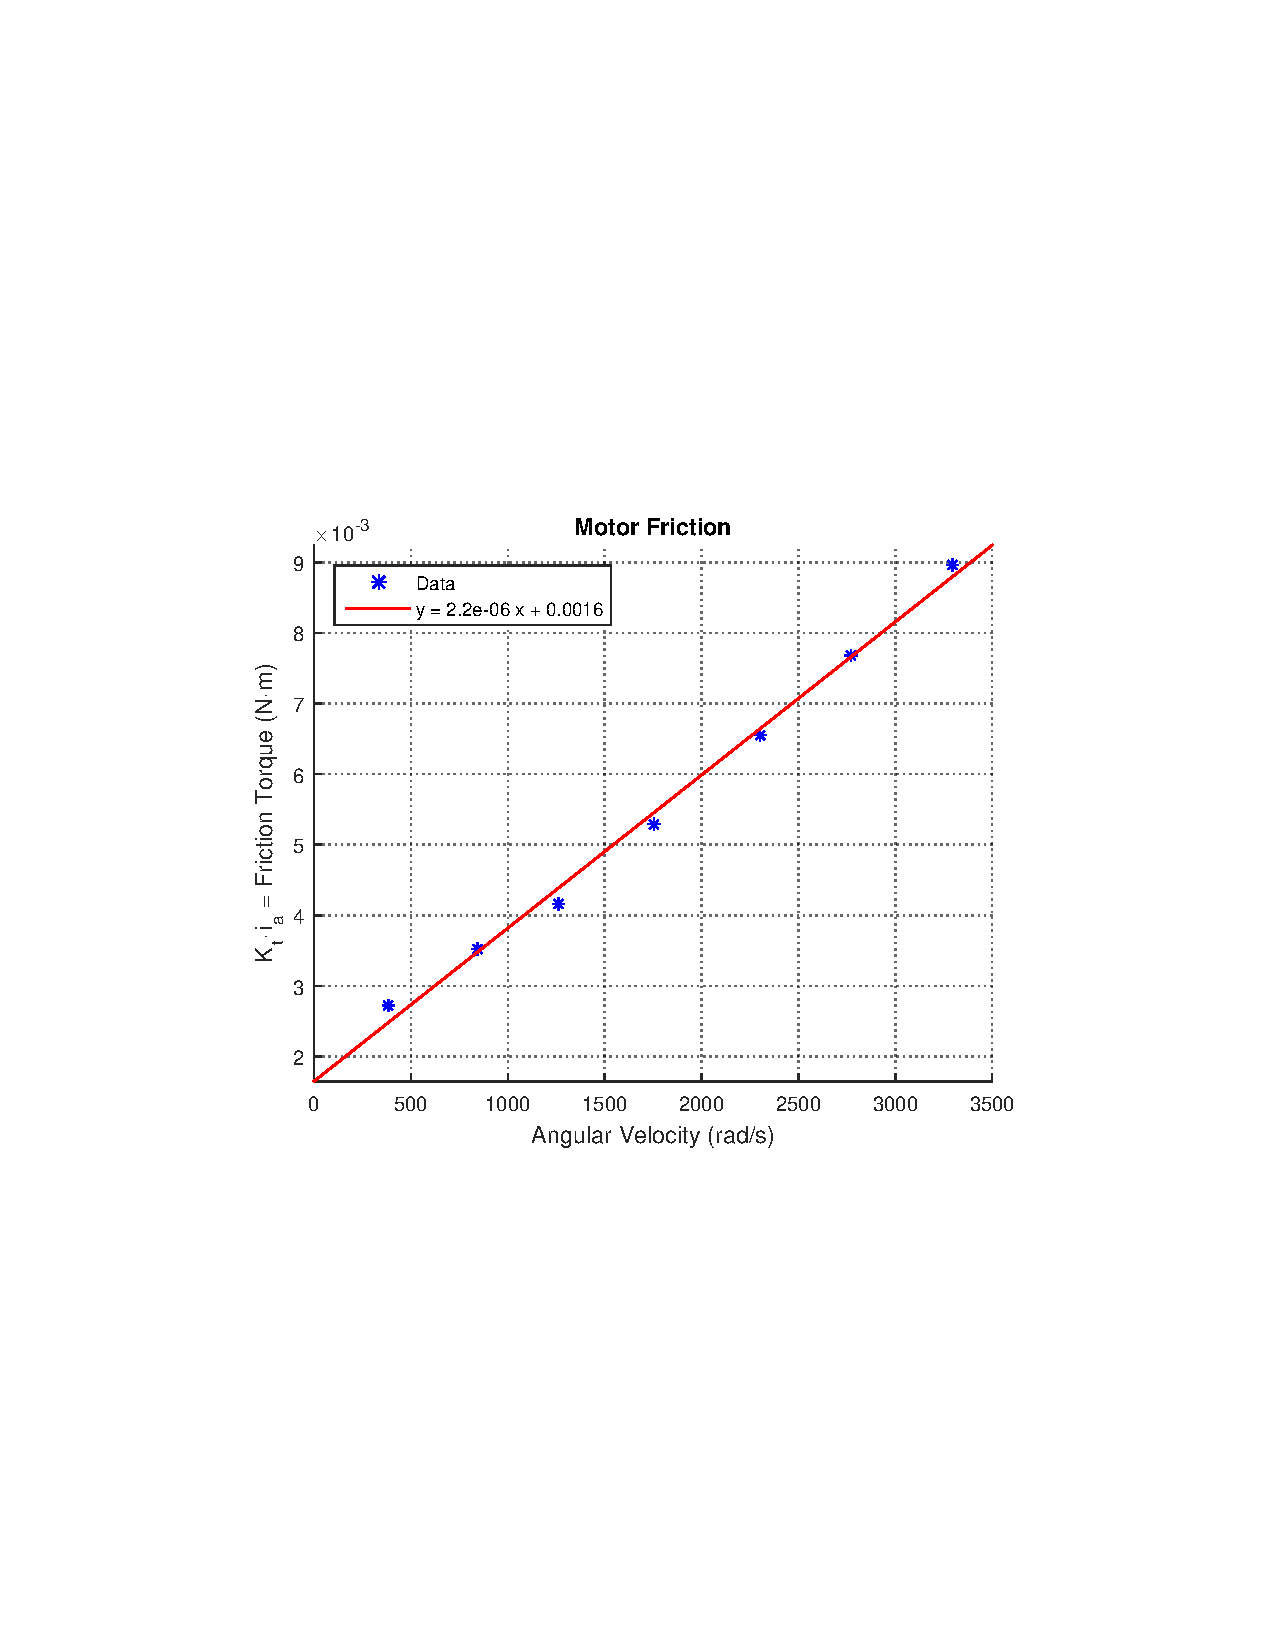
\includegraphics[width=\textwidth]{figures/motorFriction.pdf}
  }
	\caption{A plot illustrating the motor constant multiplied by the armature current to give the friction torque, which is plotted as a function of the angular velocity. The blue dots indicates the measurements and the red line indicates the least square line.}
	\label{motorFriction}
\end{figure}\vspace{-5mm}
\newpage
The following equation is applied to obtain the motor friction:

\begin{flalign}
  \eq{B}{\frac{K_t \cdot I_a}{\omega}} \unit{N\cdot m \cdot rad^{-1} \cdot s}\nonumber
\end{flalign}

\hspace{6mm} Where:\\
\begin{tabular}{p{1cm}lll}
  & \si{K_t}   & is the motor constant          &\unitWh{N\cdot m \cdot A^{-1}}           \\
  & \si{I_a}   & is the armature current        &\unitWh{A}                               \\
  & \si{B}     & is the motor friction          &\unitWh{N\cdot m \cdot rad^{-1} \cdot s} \\
  & \si{\omega}& is the motor angular velocity  &\unitWh{rad\cdot s ^{-1}}                \\
\end{tabular}

This relationship is plotted in \figref{motorFriction} and a least square line is added. The friction, B, is found as the slope and the Coulomb friction (stiction), \si{\tau_c}, is the interception between the least square line and the y-axis.

\begin{flalign}
  \eq{B}{\num{2,2}\cdot 10^{-6}} \ \si{N\cdot m \cdot rad^{-1} \cdot s}&\nonumber\\
  \eq{\tau_c}{\num{0.0016}} \ \si{N\cdot m}&\nonumber
\end{flalign}